\chapter{REVISIÓN DE LITERATURA}

\section{ANTECEDENTES DE LA INVESTIGACIÓN}

\subsection{Antecedentes internacionales}

Por otro lado, al revisar los antecedentes nos encontramos con el valioso aporte de Abou Elasaad et al. (2025), quienes en su artículo 	extit{AegisGuard: A Multi-Stage Hybrid Intrusion Detection System with Optimized Feature Selection for Industrial IoT Security} llevaron a cabo un interesante estudio experimental pensado específicamente para fortalecer la seguridad en los ecosistemas industriales (IIoT) a través de arquitecturas de análisis secuencial, implementando para ello un modelo modular de múltiples etapas llamado AegisGuard que se encarga de filtrar los flujos maliciosos aplicando una selección dinámica de características, logrando demostrar empíricamente con sus resultados que este tipo de enfoque estratificado supera con creces a los sistemas tradicionales de una sola etapa al momento de neutralizar ciberataques estructuralmente complejos, lo cual respalda por completo nuestra idea de que el camino correcto es construir arquitecturas híbridas y multicapa; sin embargo, este trabajo también nos dejó ver un detalle importante: su propuesta no logra resolver de manera principal el grave problema del sesgo algorítmico provocado por aquellas clases minoritarias que se encuentran subrepresentadas en la capa de entrada, un vacío verdaderamente crítico que justamente nuestra tesis se encargará de solucionar de raíz aplicando el algoritmo Borderline-SMOTE.

Siguiendo con la revisión de la literatura, nos topamos con el excelente trabajo de Adewole et al. (2025), quienes en su investigación 	extit{Intrusion Detection Framework for Internet of Things with Rule Induction for Model Explanation} decidieron ejecutar un diseño experimental muy interesante buscando integrar capacidades de explicabilidad dentro de los sistemas de ciberseguridad IoT, utilizando para ello los reconocidos conjuntos de datos CIC-IDS2017 y CICIoT2023 con el fin de poner a prueba el rendimiento de potentes algoritmos de Gradient Boosting, incluyendo a XGBoost, LightGBM y CatBoost. Sus resultados lograron demostrar la indiscutible superioridad técnica de XGBoost, el cual alcanzó una asombrosa exactitud (Accuracy) del 99.91\% en el primer dataset y del 98.54\% en el CICIoT2023, sumado a un AUC-ROC global del 93.06\%, lo cual justifica de manera sumamente rigurosa nuestra decisión de elegir a XGBoost como un excelente y competente algoritmo base para nuestro modelo; sin embargo, al analizarlo de cerca, notamos que este trabajo tampoco llega a implementar técnicas de rebalanceo avanzado para tratar los datos, un requisito metodológico que consideramos absolutamente indispensable para lidiar con problemas del mundo real y que justamente nuestra investigación se encargará de resolver a fondo.

Ahmed et al. (2024), en 	extit{An optimized ensemble model with advanced feature selection for network intrusion detection}, realizaron un estudio de nivel explicativo con el objetivo de optimizar la identificación de amenazas mediante la hibridación de algoritmos predictivos. La metodología consistió en integrar los modelos XGBoost y LightGBM bajo una arquitectura de ensamble tipo Stacking, evaluando el impacto de la remoción de atributos irrelevantes en la estabilidad sistémica. Los resultados confirmaron que la mitigación del ruido de entrada acelera significativamente el entrenamiento e incrementa la precisión global del clasificador. La relevancia de esta investigación radica en validar la efectividad estructural del modelo Stacking seleccionado; sin embargo, carece de un enfoque orientado específicamente a métricas de ataques minoritarios, dimensión que será el núcleo de evaluación del modelo propuesto en esta tesis.

Al-Emari et al. (2024), en su artículo 	extit{Employing Mutual Information Feature Selection and LightGBM for Intrusion Detection in IoT}, desarrollaron una investigación aplicada cuyo objetivo fue optimizar los mecanismos de protección de redes mediante la selección heurística de características. Metodológicamente, emplearon el algoritmo LightGBM evaluado sobre el conjunto de datos IoTID20, integrando el análisis de Información Mutua y la optimización por enjambre de partículas. Los resultados revelaron que esta configuración supera a las técnicas convencionales en las métricas de exactitud, sensibilidad y F1-Score, reduciendo simultáneamente la tasa de falsos positivos. Este estudio demuestra la eficacia del clasificador LightGBM para entornos IoT; sin embargo, al utilizar un dataset genérico y optimizaciones de alto costo, deja un vacío técnico que la presente tesis cubrirá mediante el dataset CICIoT2023.

Almotairi et al. (2024), en 	extit{Enhancing intrusion detection in IoT networks using machine learning-based feature selection and ensemble models}, desarrollaron una investigación aplicada sobre la gestión algorítmica ante la alta heterogeneidad del tráfico en sistemas IoT. Su protocolo metodológico consistió en acoplar modelos de ensamble clásicos, como Random Forest y Gradient Boosting, con rutinas selectivas de atributos. Los hallazgos revelaron que una discriminación óptima de variables permite a las arquitecturas mantener tasas de exactitud excepcionales garantizando baja demanda de hardware de procesamiento. Este trabajo consolida la viabilidad de utilizar algoritmos basados en árboles de decisión en ecosistemas restrictivos; no obstante, carece de evaluación sobre conjuntos de ultra-alta dimensionalidad modernos, limitación que se superará al integrar el modelo con los 46 millones de flujos del CICIoT2023.

Alrayes et al. (2024), en 	extit{Intrusion Detection in IoT Systems Using Denoising Autoencoder}, desarrollaron una investigación aplicada enfocada en la seguridad para ecosistemas IoT sujetos a alta variabilidad y recursos limitados. Utilizaron Autoencoders de Eliminación de Ruido (DAE) basados en aprendizaje no supervisado para la extracción de características, validando el sistema con los conjuntos de datos CICIDS2017 y NSL-KDD. Los resultados exhibieron precisiones sobresalientes del 99.991\% y 99.4\% respectivamente, demostrando alta fiabilidad en el procesamiento de eventos en tiempo real. Este trabajo resalta la relevancia de filtrar atributos para entornos de bajo consumo; sin embargo, su fundamentación en redes neuronales valida la propuesta de la presente tesis de integrar enfoques Stacking más ligeros para garantizar latencias de inferencia de rango inferior.

Berguiga et al. (2025), en 	extit{HIDS-IoMT: A Deep Learning-Based Intelligent Intrusion Detection System for the Internet of Medical Things}, plantearon un estudio experimental orientado a proteger redes de dispositivos médicos operando sobre arquitecturas computacionales de niebla. Metodológicamente combinaron redes convolucionales (CNN) y recurrentes (LSTM) para clasificar anomalías, ejecutando evaluaciones sobre los conjuntos de datos IoTID20 y Edge-IIoTset. Los hallazgos mostraron métricas críticas de Accuracy (99.92\%) y Recall (99.99\%) ante ataques disruptivos como denegación de servicio. Este antecedente subraya la robustez de los modelos híbridos para infraestructuras IoT de misión crítica; sin embargo, se enfoca primordialmente en ataques volumétricos mayores, dejando un área de oportunidad técnica en la identificación estricta de ataques minoritarios encubiertos.

Gutierrez et al. (2023) trabajaron en el problema de la generalización en la detección de intrusiones y para eso crearon un nuevo dataset balanceado llamado IDSAI. Con este conjunto de datos probaron varios algoritmos supervisados, entre ellos XGBoost, Gradient Boosting y Random Forest, evaluando su rendimiento frente a diez tipos distintos de ataques. Al final, XGBoost fue el que mejor desempeño mostró, alcanzando una exactitud del 94.97\% en la clasificación binaria. Lo interesante es que el modelo también se mantuvo sólido fuera del entorno de entrenamiento, porque al probarlo con el dataset externo Bot-IoT logró un 90\% de precisión, lo que demuestra que su capacidad de generalización es bastante buena.

Shanmugam et al. (2025) trabajaron el problema del desbalance de clases en ciberseguridad y para eso hicieron un análisis bastante amplio usando distintos clasificadores junto con técnicas de remuestreo como SMOTE y ADASYN. Lo que encontraron fue que aplicar estas técnicas realmente ayuda a detectar mejor los ataques que casi no aparecen en los datos, y lo bueno es que esto no afecta el rendimiento general del modelo. En resumen, su estudio muestra que el sobremuestreo no es solo un complemento, sino una parte necesaria cuando se trabaja con datasets de tráfico de red que suelen venir muy sesgados.

Nigar y Mustafa (2025) trabajaron en mejorar la detección de intrusiones poniendo énfasis en la calidad de los datos antes del entrenamiento. Con este propósito, desarrollaron un enfoque híbrido que combina técnicas de limpieza de ruido con métodos de resampling como SMOTE, logrando equilibrar las clases y optimizar el rendimiento de clasificadores tradicionales y de ensamble. En consecuencia, sus resultados evidenciaron que este tratamiento previo reduce los falsos positivos y aumenta la estabilidad de los modelos frente a ataques nuevos, incluso cuando se utilizan algoritmos como XGBoost y LightGBM. Cabe mencionar que, aunque no emplearon la entropía directamente, su estudio demuestra que el rebalanceo de datos es un componente esencial para mejorar la detección de ataques minoritarios, aportando de esta forma un antecedente clave para investigaciones que buscan integrar técnicas de optimización y ensamble en redes IoT.

Abou et al. (2025) desarrollaron AegisGuard, un sistema pensado para el IoT Industrial que funciona en varias etapas. La idea es que el modelo vaya filtrando y clasificando el tráfico malicioso paso a paso, usando una selección de características optimizada para mejorar el rendimiento. Cuando lo compararon con sistemas de una sola etapa, AegisGuard salió mejor parado, sobre todo frente a ataques más complejos. Su estudio muestra que las arquitecturas híbridas y modulares son mucho más efectivas para proteger infraestructuras críticas en el IIoT.

Tosi y Pazzi (2025) propusieron un marco híbrido denominado (H-DIR)$^2$ para la detección de anomalías y ciberseguridad en centros de datos IoT basados en la nube. Su enfoque combina el análisis de la entropía de Shannon con redes neuronales y razonamiento semántico para lograr una detección adaptativa y de baja latencia frente a ataques como inundaciones TCP SYN y manipulación de enrutamientos. En sus experimentos, los resultados evidenciaron una alta capacidad para reducir la incertidumbre en predicciones dudosas y reaccionar eficazmente en tiempo real. Este trabajo sirve como un fuerte respaldo teórico para la presente investigación, ya que confirma empíricamente que la integración de la métrica de entropía mejora notablemente la discriminación de ataques complejos y ocultos en entornos IoT.

Rahaman y Mohamad Idris (2026) desarrollaron un marco de aprendizaje por ensamble llamado STL-Net para detectar amenazas y anomalías de consumo a gran escala en infraestructuras inteligentes. Para su experimentación, integraron clasificadores ligeros como XGBoost, LightGBM, CatBoost y NGBoost bajo una arquitectura de apilamiento (Stacking), aplicando adicionalmente la técnica de rebalanceo de clases SMOTE-Tomek para lidiar con la fuerte asimetría de los datos originales. El modelo propuesto alcanzó un F1-Score del 94.47\% y un ROC-AUC del 98.69\%, demostrando ser altamente eficiente frente a clasificadores tradicionales. Este estudio aporta un antecedente metodológico directo, ya que valida el éxito de combinar arquitecturas Stacking usando XGBoost y LightGBM junto a técnicas de sobremuestreo sintético (SMOTE) para optimizar el rendimiento y neutralizar el desbalance de clases.

Peng, Wu y Xiao (2023) abordaron la problemática del desbalance de clases en la detección de intrusiones de red mediante el diseño del modelo CBF-IDS, el cual integra redes neuronales convolucionales (CNN) y BiLSTM. En lugar de modificar los datos desde su origen estadístico, su enfoque mitigó el sesgo hacia las clases mayoritarias utilizando la función de pérdida Focal Loss, evaluando su eficacia en el dataset CIC-IDS2017. Su investigación demostró que priorizar el aprendizaje de los algoritmos sobre los vectores de ataque minoritarios logra mejorar sustancialmente las tasas de detección globales. Este antecedente resulta de gran relevancia porque reafirma la necesidad crítica de tratar el desbalance de los datos para lograr identificar intrusiones poco frecuentes de forma certera, justificando plenamente la elección de integrar un preprocesamiento sólido como Borderline-SMOTE en la etapa inicial.

Neto et al. (2023) trabajaron en la creación y validación oficial del dataset CICIoT2023, con el propósito de proporcionar a la comunidad científica un entorno de referencia realista para enfrentar ataques a gran escala en redes del Internet de las Cosas. En su estudio, los investigadores documentaron 33 variantes de ataques provenientes de topologías IoT físicas, y evaluaron el desempeño base de varios algoritmos de aprendizaje automático estandarizados para clasificar el tráfico malicioso frente al benigno. Este trabajo constituye un pilar fundamental para esta tesis, ya que fundamenta las características de diseño, las representaciones minoritarias y la alta complejidad estructural del conjunto de datos sobre el cual se entrenará y pondrá a prueba el modelo híbrido de ensamble.

Katsura et al. (2025) desarrollaron un sistema de detección de intrusiones ligero para redes IoT basando su enfoque analítico en la agregación de datos por host y el uso de múltiples medidas de entropía. Su propuesta comprobó que, al representar los comportamientos del tráfico de red mediante métricas de entropía, resulta posible disminuir el consumo de memoria RAM en un 86.4\% y reducir el tiempo de respuesta drásticamente, logrando mantener una exactitud del 99.97\% empleando el algoritmo XGBoost. Los hallazgos de este artículo sustentan técnica y operativamente la investigación, al demostrar empíricamente que la sinergia entre los cálculos de entropía y los potentes modelos de Gradient Boosting garantiza una alta eficacia sin sacrificar la viabilidad computacional.

Tanveer et al. (2025) propusieron LightEnsemble-Guard, un marco de aprendizaje de ensamble optimizado con el objetivo de asegurar dispositivos IoT con recursos limitados frente a ciberataques de flujo continuo. Su metodología consistió en fusionar tres clasificadores de alto rendimiento pero de bajo peso computacional: LightGBM, XGBoost y Extra Trees, utilizando votación mayoritaria para gestionar entornos de datos desbalanceados con una alta efectividad operativa. Al conseguir una exactitud del 99.55\% superando holgadamente a los enfoques tradicionales, este trabajo documenta que la hibridación simultánea de LightGBM y XGBoost en modelos de ensamble ofrece ventajas inigualables. Por consiguiente, este estudio provee el respaldo directo y contemporáneo más sólido para justificar la integración algorítmica y la arquitectura Stacking del proyecto de tesis.

\subsection{Antecedentes nacionales}

Raico Gallardo (2025) trabajó con el dataset CICIoT2023 —el mismo que usamos en esta investigación— para evaluar qué tan bien funcionaban distintos algoritmos al clasificar tráfico IoT. Probó Naive Bayes, K Nearest Neighbors y Random Forest, aplicando antes un preprocesamiento para manejar la complejidad del dataset. Al final, el que mejor rendimiento tuvo fue Random Forest, que alcanzó una exactitud del 99.6\%. Este resultado es importante porque marca un estándar bastante alto para la detección de ataques en entornos locales y deja claro que, al menos en este caso, Random Forest supera ampliamente a los otros modelos evaluados.

Concha Ramos (2024) buscó mejorar la detección de intrusos usando Redes Neuronales Convolucionales (CNN) combinadas con Aprendizaje por Transferencia. Trabajó con el dataset UNSW-NB15 y comparó modelos entrenados desde cero con otros que ya venían pre-entrenados. Los resultados mostraron que el enfoque de transferencia fue el que mejor funcionó, logrando una precisión del 85.22\%. Esto demuestra que aprovechar el conocimiento previo de modelos profundos no solo acelera el entrenamiento, sino que también mejora la capacidad del sistema para reconocer amenazas nuevas frente a las CNN tradicionales.

Villarroel Enriquez (2025) realizó un estudio sobre malware móvil ejecutando aplicaciones maliciosas en un entorno sandbox para observar su comportamiento. Luego evaluaron distintos clasificadores, entre ellos SVM, Random Forest y LightGBM. Este último fue el que destacó, alcanzando una precisión del 94.1\% y una exactitud del 93.9\%. Sus resultados confirman que los modelos basados en Gradient Boosting son bastante efectivos para resolver problemas complejos de ciberseguridad en el contexto nacional.

Vilca et al. (2025) desarrolló un sistema inteligente para monitorear los registros (logs) de equipos IoT con el fin de detectar accesos no autorizados en infraestructuras críticas. Su propuesta se basó en técnicas de minería de datos para identificar, en tiempo real, cualquier comportamiento que se desviara de lo normal. En las pruebas piloto, el sistema logró una capacidad de detección superior al 90\%, lo que demuestra que vigilar los eventos internos de los dispositivos es tan importante como analizar el tráfico de red externo para mantener una seguridad completa.

Curioso Mercado y Gonza Callenova (2025) se enfocaron en la detección de ransomware analizando características relacionadas con el cifrado. Usaron algoritmos supervisados y el modelo que mejor funcionó fue Random Forest, que alcanzó una tasa de detección del 97.71\% con pocos falsos positivos. Este resultado confirma que el aprendizaje automático es una herramienta útil y proactiva para enfrentar ataques de ransomware que pueden afectar seriamente a empresas peruanas.

Aunque su estudio no fue sobre ciberseguridad, Oblitas Mantilla y Escobedo Cárdenas (2024) trabajaron con datos ambientales en Lima y demostraron que XGBoost y LightGBM superan a los modelos tradicionales cuando se trata de manejar grandes volúmenes de información. Obtuvieron un coeficiente de determinación mayor a 0.90, lo que muestra que estos algoritmos de ensamble son rápidos, precisos y muy eficientes. Por eso, sus resultados también sirven como respaldo técnico para elegir estas herramientas en investigaciones locales que requieren un alto rendimiento.

La presente investigación se fundamenta en la convergencia de técnicas avanzadas de aprendizaje automático para resolver vulnerabilidades críticas en infraestructuras conectadas. A continuación, se analizan las referencias teóricas y antecedentes que sustentan metodológicamente cada uno de los objetivos de este estudio.



\section{Marco Teórico}

\subsection{Internet de las Cosas (IoT)}

\subsubsection{Arquitectura distribuida y capas de red}
El paradigma del Internet de las Cosas (IoT) representa un ecosistema de computación omnipresente compuesto por objetos físicos y nodos interconectados con capacidades de detección, procesamiento y comunicación autónoma (Berguiga et al., 2025; Ferrag et al., 2022). La arquitectura de referencia estandarizada por la Unión Internacional de Telecomunicaciones (ITU-T) y el IEEE se estructura formalmente en cuatro capas funcionales interdependientes:
\begin{enumerate}
    \item \textbf{Capa de Percepción (Sensado):} Integrada por elementos de hardware de bajo nivel (sensores de temperatura, cámaras IP, actuadores domóticos, dispositivos biomédicos y microcontroladores). Su función principal radica en la adquisición continua de magnitudes del entorno físico y la conversión analógico-digital de datos (Alrayes et al., 2024).
    \item \textbf{Capa de Red y Transporte:} Responsable de la encapsulación, direccionamiento y transmisión confiable de los paquetes de tráfico. Utiliza protocolos de transporte livianos (UDP, TCP) y esquemas de red orientados a la escasez de recursos como IPv6 sobre redes inalámbricas de área personal de baja potencia (6LoWPAN), CoAP (\textit{Constrained Application Protocol}), MQTT (\textit{Message Queuing Telemetry Transport}) y Zigbee (Ahmed et al., 2024).
    \item \textbf{Capa de Niebla y Borde (\textit{Edge/Fog Computing}):} Constituida por pasarelas de red (\textit{IoT Gateways}), concentradores domóticos y servidores locales de borde. Esta capa proporciona capacidad de cómputo intermedia a baja latencia, actuando como un filtro de seguridad en tiempo real antes de enviar la información a la infraestructura central (Berguiga et al., 2025).
    \item \textbf{Capa de Aplicación y Nube:} Entorno de computación centralizado donde se ejecutan plataformas de almacenamiento masivo (*Big Data*), cuadros de mando empresarial y modelos analíticos de horizonte temporal extendido.
\end{enumerate}

\begin{figure}[H]
\centering
\caption{Arquitectura distribuida de cuatro capas funcionales en entornos IoT}
\label{fig:arquitectura_iot_capas_exp}
\begin{tikzpicture}[
    node distance=0.6cm,
    layer/.style={rectangle, draw=blue!80!black, fill=blue!6, thick, text width=12.5cm, minimum height=0.9cm, align=center, rounded corners=3pt},
    arrow/.style={<->, >=stealth, thick, draw=blue!80!black}
]

\node[layer, fill=purple!10, draw=purple!80!black] (l4) {\textbf{Capa 4: Aplicación y Nube} \\ Servicios analíticos, gestión domótica, plataformas empresariales y almacenamiento masivo};
\node[layer, fill=cyan!10, draw=cyan!80!black, below=of l4] (l3) {\textbf{Capa 3: Niebla y Borde (\textit{Edge/Fog Computing})} \\ Pasarelas IoT (\textit{Gateways}), servidores locales de borde y motores de inferencia en tiempo real};
\node[layer, fill=orange!10, draw=orange!80!black, below=of l3] (l2) {\textbf{Capa 2: Red y Transporte} \\ Protocolos de comunicación (TCP/IP, UDP, IPv6/6LoWPAN, MQTT, CoAP, Wi-Fi, Zigbee)};
\node[layer, fill=green!10, draw=green!80!black, below=of l2] (l1) {\textbf{Capa 1: Percepción y Captura} \\ Sensores físicos, actuadores, cámaras IP, termostatos y microcontroladores integrados};

\draw[arrow] (l1) -- (l2);
\draw[arrow] (l2) -- (l3);
\draw[arrow] (l3) -- (l4);

\end{tikzpicture}
\end{figure}

\subsubsection{Dispositivos de borde y pasarelas IoT (IoT Gateways)}
En la capa de borde (\textit{Edge/Fog Computing}), las pasarelas de red (\textit{IoT Gateways}) operan como nodos concentradores y puntos de inspección obligatorios (Ferrag et al., 2022). Dado que estos dispositivos agregan el tráfico de docenas de micro-nodos y convierten protocolos heterogéneos a tramas Ethernet/IP estándar, constituyen la posición estratégica idónea para desplegar Sistemas de Detección de Intrusiones (IDS) locales (Alrayes et al., 2024; Raico Gallardo, 2025). El procesamiento local en pasarelas evita el costo operativo de transmitir gigabytes de tráfico sin filtrar hacia la nube, garantizando resiliencia funcional ante la pérdida eventual de conectividad a Internet.

\subsubsection{Restricciones computacionales, de memoria y latencia}
A pesar de su criticidad estratégica, las pasarelas y nodos de borde en entornos IoT exhiben restricciones de hardware severas que condicionan la elección del modelo analítico (Ahmed et al., 2024; Almotairi et al., 2024):
\begin{enumerate}
    \item \textbf{Memoria RAM acotada:} Las pasarelas de borde industriales y comerciales disponen de memorias volátiles limitadas (típicamente entre 512 MB y 4 GB de RAM). Las arquitecturas de aprendizaje profundo masivas (como CNNs complejas o Transformers de redes) superan este umbral provocando fallos por memoria insuficiente (\textit{Out-Of-Memory}).
    \item \textbf{Capacidad de procesamiento CPU:} Microprocesadores integrados (arquitecturas ARM Cortex v7/v8 o x86 de bajo consumo) de baja frecuencia de reloj, lo que exige algoritmos de baja complejidad temporal $\mathcal{O}(N \log N)$.
    \item \textbf{Presupuesto de latencia ultrabaja:} En la gestión de tráfico de red, la clasificación de cada flujo debe resolverse en microsegundos ($\mu s$). Una latencia elevada provocaría congestión de búferes y pérdida masiva de paquetes legítimos (Kouassi et al., 2025b).
\end{enumerate}

\subsubsection{Protocolos de comunicación de transporte (TCP/IP vs. UDP)}
El comportamiento del tráfico de red en IoT está fuertemente condicionado por la elección del protocolo del nivel de transporte (Adewole et al., 2025). Mientras que el protocolo TCP (\textit{Transmission Control Protocol}) garantiza la entrega mediante apretones de manos de tres vías (\textit{Three-Way Handshake}) y control de flujo, el protocolo UDP (\textit{User Datagram Protocol}) prioriza la velocidad y la baja latencia sin confirmación de recepción. Esta dicotomía es explotada por los ciberatacantes: los ataques volumétricos emplean inundaciones UDP o SYN para agotar la memoria de estados, mientras que los ataques a nivel de aplicación emplean sesiones TCP establecidas para inyectar vectores maliciosos de baja frecuencia (Ferrag et al., 2022).

\subsection{Ciberseguridad y Detección de Intrusiones}

\subsubsection{Sistemas de Detección de Intrusiones (IDS)}
Un Sistema de Detección de Intrusiones (IDS) es un mecanismo de defensa en profundidad diseñado para analizar continuamente el flujo de paquetes de red, identificando patrones anómalos, firmas de ataque o desviaciones de la conducta normal (Adewole et al., 2025; Musthafa et al., 2024). Los IDS se clasifican operacionalmente en dos categorías:
\begin{itemize}
    \item \textbf{IDS Basados en Firmas (\textit{Signature-based IDS}):} Comparan el tráfico entrante contra reglas estáticas conocidas (como Snort o Suricata). Son ineficaces frente a ataques emergentes o variaciones de día cero (*Zero-Day*).
    \item \textbf{IDS Basados en Anomalías y Machine Learning (\textit{Anomaly-based IDS}):} Construyen modelos estadísticos y probabilísticos a partir de datos históricos, permitiendo generalizar y detectar patrones anómalos nunca antes vistos.
\end{itemize}

\subsubsection{Arquitecturas NIDS vs. HIDS}
Atendiendo a la ubicación de despliegue, la literatura distingue entre Sistemas de Detección de Intrusiones Basados en Host (\textit{HIDS - Host Intrusion Detection System}), que inspeccionan llamadas al sistema y logs de auditoría en un único dispositivo; y Sistemas de Detección de Intrusiones Basados en Red (\textit{NIDS - Network Intrusion Detection System}), los cuales analizan la cabecera y las métricas estadísticas de las ráfagas de paquetes que atraviesan los enlaces de comunicación (Berguiga et al., 2025). La presente tesis se posiciona en el paradigma NIDS, inspeccionando vectores de atributos estadísticos extraídos de los flujos IP.

\subsubsection{Caracterización del tráfico con el dataset CICIoT2023}
El desarrollo y validación experimental de esta investigación se fundamenta en el conjunto de datos estandarizado internacional \textbf{CICIoT2023}, publicado por el \textit{Canadian Institute for Cybersecurity} (Adewole et al., 2025; Raico Gallardo, 2025). Este dataset fue diseñado capturando la actividad en una topología física real compuesta por 33 dispositivos IoT (cámaras IP, altavoces domóticos, sensores, concentradores) sometidos a 33 vectores de ciberataque ejecutados bajo escenarios realistas.

El espacio vectorial original comprende 47 características estadísticas de red. Tras el proceso de selección de atributos por impureza de Gini e Información Mutua, el espacio de entrada se redujo a $d=29$ variables continuas (tasas de paquetes por segundo, duración de flujos, tiempo entre llegadas, tamaño de cabeceras, indicadores de bandera TCP, varianza de tamaño de paquete, entre otros). El espacio categórico de salida se define como el conjunto de 8 clases de tráfico:
\begin{equation}
\mathcal{Y} = \{\mathrm{Benign}, \mathrm{Brute\ Force}, \mathrm{DDoS}, \mathrm{DoS}, \mathrm{Mirai}, \mathrm{Reconnaissance}, \mathrm{Spoofing}, \mathrm{Web\text{-}based}\}
\end{equation}

\subsubsection{Taxonomía de ciberataques: Volumétricos vs. Minoritarios}
Desde la perspectiva de la distribución cuantitativa del volumen de tráfico, los ataques cibernéticos se dividen en dos grandes familias taxonómicas (Ferrag et al., 2022; Nigar \& Mustafa, 2025):
\begin{enumerate}
    \item \textbf{Ataques Volumétricos Dominantes (\textit{DDoS}, \textit{DoS}, \textit{Mirai Botnet}):} Caracterizados por la emisión masiva de ráfagas de datos diseñadas para saturar la capacidad de procesamiento de la red. Representan el $95.53\%$ de los registros anómalos del dataset CICIoT2023. Incluyen inundaciones UDP (\textit{UDP Flood}), inundaciones SYN (\textit{TCP SYN Flood}), inundaciones ICMP y ataques distribuidos coordinados por botnets infectadas como Mirai.
    \item \textbf{Ataques Minoritarios Infrecuentes y Sigilosos (\textit{Web-based}, \textit{Brute Force}, \textit{Reconnaissance}):} Caracterizados por secuencias extremadamente reducidas en número de paquetes ($<0.5\%$ del volumen global) pero con un grado de amenaza destructiva crítico:
    \begin{itemize}
        \item \textit{Web-based Attacks:} Inyecciones SQL (\textit{SQLi}), ejecución remota de comandos (\textit{Command Injection}) y secuencias de comandos entre sitios (\textit{XSS}) dirigidas a interfaces web de gestión en dispositivos domóticos.
        \item \textit{Brute Force Attacks:} Intentos automatizados y sistemáticos de adivinación de credenciales sobre servicios de acceso remoto SSH y Telnet.
        \item \textit{Reconnaissance:} Escaneo de puertos abiertos (*PortScan*) y análisis de huella digital de sistemas operativos (*OS Fingerprinting*) para descubrir vulnerabilidades explotables.
    \end{itemize}
\end{enumerate}

\subsection{Desbalance de Datos y Preprocesamiento}

\subsubsection{Teorema del No Free Lunch y Desbalance de Clases}
En la Teoría del Aprendizaje Estadístico, el Teorema del *No Free Lunch* (Wolpert, 1996) establece que ningún algoritmo de clasificación es universalmente superior sobre todas las distribuciones de probabilidad posibles. Cuando la distribución a priori de las clases objetivo $P(Y=k)$ presenta una asimetría extrema, los algoritmos supervisados convencionales colapsan en su capacidad discriminativa (Shanmugam et al., 2025).

\subsubsection{Índice de Desbalance (Imbalance Ratio - IR)}
Sea $S_k = \{x_i \in D \mid y_i = k\}$ el subconjunto de instancias pertenecientes a la categoría $k \in \mathcal{Y}$. El Índice de Desbalance (\textit{Imbalance Ratio - IR}) mide formalmente la desproporción cuantitativa entre la clase más frecuente y la menos frecuente (Kouassi et al., 2025a):
\begin{equation}
\mathrm{IR} = \frac{\max_{k \in \mathcal{Y}} |S_k|}{\min_{k \in \mathcal{Y}} |S_k|}
\end{equation}
En el conjunto de prueba aislado de la investigación ($N_{\mathrm{test}} = 377,383$ muestras), la clase mayoritaria DDoS registra $|S_{\mathrm{DDoS}}| = 148,475$ observaciones, mientras que la clase minoritaria crítica \textit{Web-based} cuenta con apenas $|S_{\mathrm{Web\text{-}based}}| = 3,556$ observaciones, arrojando un ratio extremo de:
\begin{equation}
\mathrm{IR} = \frac{148,475}{3,556} \approx 41.75
\end{equation}

\subsubsection{Sesgo algorítmico y Paradoja de la Exactitud (Accuracy Paradox)}
Durante la fase de optimización de los parámetros del modelo, los clasificadores supervisados buscan minimizar la función de pérdida empírica global:
\begin{equation}
\mathcal{L}_{\mathrm{emp}}(f) = \frac{1}{N} \sum_{i=1}^N l(y_i, f(x_i))
\end{equation}
Dado que el $95\%$ de las observaciones pertenecen a clases volumétricas mayoritarias, los gradientes de actualización del error están dominados casi exclusivamente por dichas instancias (Wu et al., 2025). Como resultado, el clasificador desplaza su hiperplano de decisión hacia la región de las clases minoritarias, clasificando erróneamente casi todas las muestras de \textit{Web-based} y \textit{Brute Force} como tráfico benigno o DoS. Esto desencadena la denominada \textit{Paradoja de la Exactitud} (\textit{Accuracy Paradox}): el sistema reporta una exactitud global falsamente elevada ($>84\%$) simplemente por predecir correctamente las clases volumétricas, pese a presentar una sensibilidad prácticamente nula ($Recall \to 0$) en la detección de los ataques infrecuentes más peligrosos (Nigar \& Mustafa, 2025).

\subsubsection{Escalado Robusto Adaptativo (RobustScaler)}
El tráfico de red en entornos IoT se caracteriza por presentar distribuciones estadísticas fuertemente sesgadas y ráfagas extremas de valores atípicos (\textit{outliers}) provocadas por los ataques volumétricos. La aplicación de técnicas de escalado tradicionales resulta inapropiada (Curioso \& Gonza, 2025):
\begin{itemize}
    \item \textbf{StandardScaler ($Z$-Score):} Fundado en la media aritmética $\mu_j$ y la desviación estándar $\sigma_j$, métricas extremadamente sensibles a valores atípicos que distorsionan el rango transformado.
    \item \textbf{MinMaxScaler:} Comprime los valores al intervalo $[0, 1]$ utilizando el mínimo y máximo absoluto, lo cual provoca que las ráfagas extremas colapsen el 99\% de los datos normales en un rango diminuto cercano a cero.
\end{itemize}

Para mitigar esta distorsión sin descartar información real, se aplica el algoritmo \textbf{RobustScaler}, el cual sustituye los momentos estadísticos por la Mediana ($Q_2$) y el Rango Intercuartílico ($\mathrm{IQR} = Q_3 - Q_1$) (Al-Emari et al., 2024):
\begin{equation}
x_{ij}^{\mathrm{scaled}} = \frac{x_{ij} - Q_2(x_j)}{Q_3(x_j) - Q_1(x_j)} = \frac{x_{ij} - \mathrm{Mediana}(x_j)}{\mathrm{IQR}(x_j)}
\end{equation}
En caso de que el rango sea nulo ($\mathrm{IQR}_j = 0$), se asigna $\mathrm{IQR}_j = 1.0$ para evitar indeterminaciones matemáticas por división sobre cero.

\subsubsection{Sobremuestreo Sintético en la Frontera (Borderline-SMOTE1)}
Para resolver el desbalance de clases sin incurrir en pérdida de información por submuestreo aleatorio (RUS), la literatura propone técnicas de sobremuestreo sintético (Sayegh et al., 2024; Shanmugam et al., 2025). No obstante, el algoritmo SMOTE convencional genera muestras sintéticas en todo el espacio minoritario de forma no discriminativa, lo que suele introducir ruido en el interior de la región de la clase mayoritaria.

Para superar esta limitación, el algoritmo \textbf{Borderline-SMOTE1} (Nigar \& Mustafa, 2025) restringe la generación sintética exclusivamente a aquellas instancias minoritarias que se ubican en la franja limítrofe o zona de peligro de decisión ($S_{\mathrm{danger}}$).

\begin{figure}[H]
\centering
\caption{Topología de frontera y generación sintética de instancias con Borderline-SMOTE1}
\label{fig:topologia_borderline_exp}
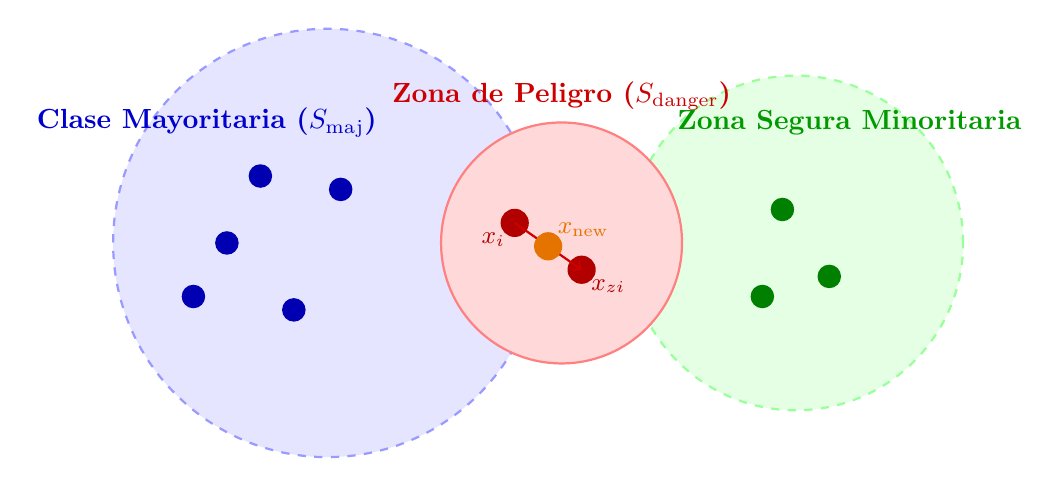
\begin{tikzpicture}[scale=0.85]

% Region Mayoritaria
\draw[fill=blue!10, draw=blue!40, dashed, thick] (0,0) circle (3.2cm);
\node[blue!80!black] at (-1.8, 1.8) {\textbf{Clase Mayoritaria ($S_{\mathrm{maj}}$)}};
\fill[blue!70!black] (-1,1) circle (5pt);
\fill[blue!70!black] (-1.5,0) circle (5pt);
\fill[blue!70!black] (-0.5,-1) circle (5pt);
\fill[blue!70!black] (-2,-0.8) circle (5pt);
\fill[blue!70!black] (0.2,0.8) circle (5pt);

% Region Minoritaria Segura
\draw[fill=green!10, draw=green!40, dashed, thick] (7,0) circle (2.5cm);
\node[green!60!black] at (7.8, 1.8) {\textbf{Zona Segura Minoritaria}};
\fill[green!50!black] (6.8,0.5) circle (5pt);
\fill[green!50!black] (7.5,-0.5) circle (5pt);
\fill[green!50!black] (6.5,-0.8) circle (5pt);

% Zona de Frontera Danger
\draw[fill=red!15, draw=red!50, thick] (3.5,0) circle (1.8cm);
\node[red!80!black] at (3.5, 2.2) {\textbf{Zona de Peligro ($S_{\mathrm{danger}}$)}};
\fill[red!70!black] (2.8,0.3) circle (6pt) node[below left]{\small $x_i$};
\fill[red!70!black] (3.8,-0.4) circle (6pt) node[below right]{\small $x_{zi}$};
\draw[thick, red!80!black, ->] (2.8,0.3) -- (3.8,-0.4);
\fill[orange!90!black] (3.3,-0.05) circle (6pt) node[above right]{\small $x_{\mathrm{new}}$};

\end{tikzpicture}
\end{figure}

El procedimiento computacional de Borderline-SMOTE1 opera secuencialmente en tres etapas sobre las muestras minoritarias $S_{\mathrm{min}}$:
\begin{enumerate}
    \item \textbf{Cálculo de Vecindad Euclidiana:} Para cada instancia minoritaria $x_i \in S_{\mathrm{min}}$, se determinan sus $m$ vecinos más cercanos en el conjunto completo de entrenamiento mediante la distancia Euclidiana:
    \begin{equation}
    d(x_i, x_j) = \sqrt{\sum_{l=1}^d (x_{il} - x_{jl})^2}
    \end{equation}
    \item \textbf{Clasificación Topológica de Instancias:} Se contabiliza el número de vecinos $m_v$ pertenecientes a la clase mayoritaria $S_{\mathrm{maj}}$:
    \begin{itemize}
        \item Si $m_v = m$, todos los vecinos son mayoritarios; la muestra se considera ruido aislado y no se sobremuestrea.
        \item Si $0 \le m_v < m/2$, la mayoría de los vecinos son minoritarios; la muestra está segura en el interior de su conglomerado ($S_{\mathrm{safe}}$) y no requiere intervención.
        \item Si $m/2 \le m_v < m$, la muestra está rodeada predominantemente por la clase mayoritaria; se clasifica como punto limítrofe en peligro ($x_i \in S_{\mathrm{danger}}$).
    \end{itemize}
    \item \textbf{Interpolación Sintética en la Frontera:} Para cada $x_i \in S_{\mathrm{danger}}$, se identifican sus $k$ vecinos más cercanos pertenecientes únicamente a la clase minoritaria $S_{\mathrm{min}}$. Se selecciona aleatoriamente un vecino $x_{zi}$ y se genera una nueva observación sintética $x_{\mathrm{new}}$ mediante la fórmula de interpolación lineal:
    \begin{equation}
    x_{\mathrm{new}} = x_i + \delta \cdot (x_{zi} - x_i), \quad \delta \sim U(0,1)
    \end{equation}
    donde $\delta$ es un escalar aleatorio generado desde una distribución uniforme continua en el intervalo $[0, 1]$.
\end{enumerate}

\subsection{Algoritmos de Aprendizaje Automático Base (Nivel 0)}

\subsubsection{Teoría de Ensamble y Compromiso Sesgo-Varianza}
En el marco del aprendizaje supervisado, el error cuadrático medio de un estimador se descompone axiomáticamente como:
\begin{equation}
\mathrm{Error}(f) = \mathrm{Sesgo}^2(f) + \mathrm{Varianza}(f) + \sigma_{\mathrm{ruido}}^2
\end{equation}
Los clasificadores individuales simples suelen sufrir de alto sesgo (subajuste) o alta varianza (sobreajuste). Los métodos de ensamble (*Ensemble Learning*) combinan múltiples clasificadores base para reducir simultáneamente la varianza (mediante *Bagging*) y el sesgo (mediante *Gradient Boosting*), alcanzando un compromiso óptimo (Zwane et al., 2019; Almotairi et al., 2024).

\subsubsection{Random Forest (Bagging e Impureza de Gini)}
Random Forest (Breiman, 2001; Almotairi et al., 2024; Kouassi et al., 2025b; Raico Gallardo, 2025) es una arquitectura de ensamble basada en *Bagging* (*Bootstrap Aggregating*). Construye $M=100$ árboles de decisión no correlacionados $\{h_m(x)\}_{m=1}^M$ entrenados sobre submuestras aleatorias obtenidas por remuestreo con reemplazo.

Para descorrelacionar los árboles, en cada división de nodo el algoritmo no evalúa la totalidad de las $d$ características, sino un subconjunto restringido de $m_{\mathrm{try}} = \sqrt{d} = \sqrt{29} \approx 5$ atributos seleccionados al azar. La probabilidad predicha para la clase $k \in \{0, \dots, 7\}$ es el promedio simple de las probabilidades emitidas por cada árbol individual:
\begin{equation}
P_{\mathrm{RF}}(Y=k | x) = \frac{1}{M} \sum_{m=1}^M P_{h_m}(Y=k | x)
\end{equation}
La selección de la mejor división en cada nodo se guía por la maximización de la ganancia de Impureza de Gini:
\begin{equation}
I_G(p) = 1 - \sum_{k=0}^{K-1} p_k^2
\end{equation}
donde $p_k$ representa la proporción de instancias pertenentes a la clase $k$ en el nodo evaluado.

\subsubsection{XGBoost GPU (Gradient Boosting regularizado de 2º orden)}
XGBoost (*Extreme Gradient Boosting*) (Chen \& Guestrin, 2016; Adewole et al., 2025; Gutierrez et al., 2023; Oblitas \& Escobedo, 2024) es un algoritmo de Gradient Boosting aditivo que construye árboles de decisión secuencialmente. En cada iteración $t$, el nuevo árbol $f_t(x)$ se añade para minimizar la siguiente función objetivo regularizada:
\begin{equation}
\mathcal{L}^{(t)} = \sum_{i=1}^N l\left(y_i, \hat{y}_i^{(t-1)} + f_t(x_i)\right) + \Omega(f_t)
\end{equation}
donde el término de regularización L1/L2 $\Omega(f_t)$ penaliza la complejidad estructural del árbol:
\begin{equation}
\Omega(f_t) = \gamma T_{\mathrm{hojas}} + \frac{1}{2}\lambda \sum_{j=1}^{T_{\mathrm{hojas}}} w_j^2
\end{equation}
siendo $T_{\mathrm{hojas}}$ el número de hojas terminales y $w_j$ el peso asignado a cada hoja.

A diferencia del Gradient Boosting clásico, XGBoost aproxima la función objetivo mediante la expansión de la serie de Taylor de segundo orden:
\begin{equation}
\mathcal{L}^{(t)} \approx \sum_{i=1}^N \left[ l(y_i, \hat{y}_i^{(t-1)}) + g_i f_t(x_i) + \frac{1}{2} h_i f_t^2(x_i) \right] + \Omega(f_t)
\end{equation}
donde los términos de primer y segundo orden corresponden al gradiente $g_i$ y al Hessiano $h_i$:
\begin{equation}
g_i = \frac{\partial l(y_i, \hat{y}^{(t-1)})}{\partial \hat{y}^{(t-1)}}, \quad h_i = \frac{\partial^2 l(y_i, \hat{y}^{(t-1)})}{\partial (\hat{y}^{(t-1)})^2}
\end{equation}
Para acelerar masivamente el procesamiento de los 2.51 millones de registros, XGBoost se ejecuta en la GPU NVIDIA RTX 5070 Ti mediante el método de construcción de histogramas cuantizados en memoria gráfica (\texttt{tree\_method='hist'}, \texttt{device='cuda'}).

\subsubsection{LightGBM (Crecimiento por hojas Leaf-wise, GOSS y EFB)}
LightGBM (*Light Gradient Boosting Machine*) (Ke et al., 2017; Al-Emari et al., 2024; Oblitas Mantilla \& Escobedo Cárdenas, 2024; Villarroel Enriquez, 2025) es un marco de trabajo de Gradient Boosting diseñado para ofrecer alta velocidad y eficiencia en memoria. Presenta tres innovaciones arquitectónicas:
\begin{enumerate}
    \item \textbf{Estrategia de Crecimiento por Hojas (\textit{Leaf-Wise Growth}):} En lugar de expandir los árboles nivel por nivel de forma simétrica (*Level-Wise*), LightGBM busca y expande de forma codiciosa la hoja con la mayor ganancia de pérdida esperada (*delta loss*), fijando un límite de profundidad (\texttt{max\_depth=6}) para evitar sobreajuste.
    \item \textbf{GOSS (\textit{Gradient-Based One-Side Sampling}):} Ordena descendentemente las instancias según el valor absoluto de su gradiente $|g_i|$. Conserva el $100\%$ de las observaciones con gradientes grandes (las más difíciles de clasificar) y realiza un muestreo aleatorio uniforme sobre las instancias con gradientes pequeños, multiplicando a estas últimas por un factor de compensación para mantener la distribución original.
    \item \textbf{EFB (\textit{Exclusive Feature Bundling}):} Empaqueta variables dispersas que son mutuamente excluyentes (es decir, que rara vez toman valores distintos de cero simultáneamente) en un menor número de características densas, reduciendo la complejidad espectral del problema.
\end{enumerate}
Las probabilidades multiclase $P_{\mathrm{LGB}}(Y=k|x)$ se obtienen aplicando la función de activación Softmax sobre las puntuaciones continuas $F_k(x)$:
\begin{equation}
P_{\mathrm{LGB}}(Y=k|x) = \frac{\exp(F_k(x))}{\sum_{j=0}^{K-1} \exp(F_j(x))}
\end{equation}

\subsection{Cuantificación de Incertidumbre Predictiva}

\subsubsection{Teoría de la Información de Shannon}
La Teoría de la Información desarrollada axiomáticamente por Claude Shannon (1948) provee las bases matemáticas para cuantificar la cantidad de incertidumbre, entropía e información contenida en una variable aleatoria discreta (Sepúlveda-Fontaine \& Amigó, 2024).

\subsubsection{Entropía de Shannon como métrica de ambigüedad predictiva}
En el contexto de la clasificación multiclase, cuando un clasificador base $m \in \{\mathrm{RF}, \mathrm{XGB}, \mathrm{LGB}\}$ evalúa un flujo de red $x$, emite un vector discreto de probabilidades $\mathbf{P}_m(x) = [p_0, p_1, \dots, p_7] \in \mathbb{R}^8$, donde $\sum_{k=0}^7 p_k = 1.0$.

La Entropía de Shannon $H_m(x)$ mide la incertidumbre o dispersión lógica inherente a dicha distribución (Diwan et al., 2022; Popoola et al., 2025; Sama et al., 2025):
\begin{equation}
H_m(x) = -\sum_{k=0}^{K-1} P_m(Y=k|x) \log_2 \left( P_m(Y=k|x) + \epsilon \right)
\end{equation}
donde $\epsilon = 10^{-15}$ es una constante infinitesimal agregada para garantizar estabilidad numérica y prevenir indeterminaciones por $\log_2(0)$.

\begin{figure}[H]
\centering
\caption{Comportamiento de la Entropía de Shannon según la dispersión del vector de probabilidad}
\label{fig:entropia_comportamiento}
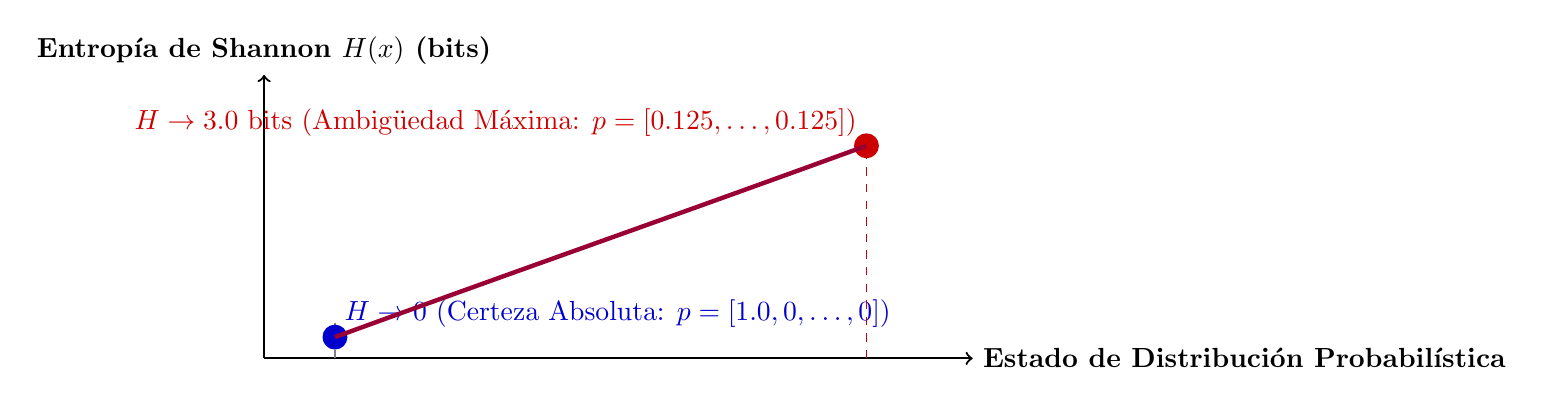
\begin{tikzpicture}[scale=0.9]

% Eje horizontal
\draw[->, thick] (0,0) -- (10,0) node[right] {\textbf{Estado de Distribución Probabilística}};
\draw[->, thick] (0,0) -- (0,4) node[above] {\textbf{Entropía de Shannon $H(x)$ (bits)}};

% Puntos limite
\draw[dashed, gray] (1,0) -- (1,0.5);
\fill[blue!80!black] (1,0.3) circle (5pt) node[above right] {$H \to 0$ (Certeza Absoluta: $p = [1.0, 0, \dots, 0]$)};

\draw[dashed, red!80!black] (8.5,0) -- (8.5,3.2);
\fill[red!80!black] (8.5,3.0) circle (5pt) node[above left] {$H \to 3.0$ bits (Ambigüedad Máxima: $p = [0.125, \dots, 0.125]$)};

% Curva conceptual
\draw[ultra thick, purple!80!black] (1,0.3) to[out=20, in=200] (8.5,3.0);

\end{tikzpicture}
\end{figure}

Las propiedades funcionales de la Entropía de Shannon son:
\begin{itemize}
    \item \textbf{Certeza Absoluta ($H_m(x) \to 0$ bits):} Ocurre cuando el clasificador base asigna $p_k \approx 1.0$ a una sola clase y $p_j \approx 0.0$ a las restantes. Indica que el modelo está completamente seguro de su predicción.
    \item \textbf{Ambigüedad Máxima ($H_m(x) \to \log_2(8) = 3.0$ bits):} Ocurre cuando el modelo asigna una probabilidad equiprobable $p_k \approx 1/8 = 0.125$ a las 8 clases. Esta condición suele manifestarse en las regiones fronterizas entre tráfico benigno y vectores de ataque minoritarios infrecuentes, alertando formalmente al meta-clasificador sobre la zona de alta duda.
\end{itemize}

\subsection{Arquitectura de Ensamble por Stacking Híbrido}

\subsubsection{Principios teóricos del Stacking (Stacked Generalization)}
La arquitectura de ensamble por Stacking (*Stacked Generalization*) fue formulada por David Wolpert (1992) como un esquema de meta-aprendizaje diseñado para deducir qué clasificadores base son más confiables en qué regiones del espacio de características (Ahmed et al., 2024; Musthafa et al., 2024; Lin et al., 2021). A diferencia de los ensambles por *Voting* (voto mayoritario) o *Averaging* (promedio simple), Stacking entrena un modelo superior de Nivel 1 (*Meta-Modelo*) que aprende a combinar de forma no lineal las salidas probabilísticas de los modelos de Nivel 0.

\subsubsection{Generación de Meta-características fuera de pliegue (OOF)}
Un desafío metodológico crítico en las arquitecturas Stacking es la prevención de la Fuga de Datos (*Data Leakage*) y el sobreajuste (*Overfitting*). Si el meta-modelo se entrena utilizando las predicciones generadas por los modelos de Nivel 0 sobre los mismos datos con los que fueron entrenados, el metamodelo memorizará el sesgo de los clasificadores primarios.

Para resolver este problema de forma científicamente rigurosa, las meta-características se construyen aplicando una validación cruzada estratificada fuera de pliegue (*Out-Of-Fold - OOF*) de $K=3$ pliegues (Musthafa et al., 2024; Nigar \& Mustafa, 2025):
\begin{enumerate}
    \item El conjunto de entrenamiento $D_{\mathrm{train}}$ se particiona en 3 subconjuntos disjuntos estratificados.
    \item En cada iteración $k \in \{1, 2, 3\}$, los clasificadores base (Random Forest, XGBoost GPU y LightGBM) se entrenan sobre 2 pliegues y emiten sus predicciones únicamente sobre el pliegue de validación retenido.
    \item Se calculan las 3 entropías de Shannon instantáneas $H_{\mathrm{RF}}, H_{\mathrm{XGB}}, H_{\mathrm{LGB}}$ sobre las probabilidades del pliegue retenido.
    \item Se concatenan las 24 probabilidades predichas ($3 \text{ modelos} \times 8 \text{ clases}$) junto con las 3 métricas de entropía, formando la matriz de meta-características $Z_{\mathrm{train}} \in \mathbb{R}^{N_{\mathrm{train}} \times 27}$:
    \begin{equation}
    z_i = \Big[ P_{\mathrm{RF}}(x_i), P_{\mathrm{XGB}}(x_i), P_{\mathrm{LGB}}(x_i), H_{\mathrm{RF}}(x_i), H_{\mathrm{XGB}}(x_i), H_{\mathrm{LGB}}(x_i) \Big] \in \mathbb{R}^{27}
    \end{equation}
\end{enumerate}

\subsubsection{Meta-Modelo de Nivel 1 (LightGBM)}
El meta-clasificador de Nivel 1 es una instancia optimizada de LightGBM que toma como espacio vectorial de entrada la matriz $Z \in \mathbb{R}^{27}$ (Ke et al., 2017; Villarroel Enriquez, 2025). Durante la fase de entrenamiento, el meta-modelo aprende patrones complejos de decisión; por ejemplo, si Random Forest presenta alta entropía ($H_{\mathrm{RF}} > 2.5$) en un flujo específico, el meta-modelo otorga mayor ponderación a la predicción de XGBoost GPU o examina las probabilidades minoritarias residuales.

La sintonización fina de los hiperparámetros del meta-modelo se ejecutó mediante una búsqueda en malla con validación cruzada (\texttt{GridSearchCV}), fijando la combinación óptima: \texttt{n\_estimators=100}, \texttt{learning\_rate=0.05}, \texttt{num\_leaves=31}, \texttt{max\_depth=6}, \texttt{subsample=0.8} y \texttt{colsample\_bytree=0.8}.

\subsection{Métricas de Evaluación y Prueba Estadística}

\subsubsection{Métricas de clasificación multiclase}
Dada la matriz de confusión de contingencia $K \times K$ ($K=8$), para cada categoría $k \in \{0, \dots, 7\}$ se definen los parámetros de conteo: Verdaderos Positivos ($TP_k$), Falsos Positivos ($FP_k$), Verdaderos Negativos ($TN_k$) y Falsos Negativos ($FN_k$) (Kouassi et al., 2025b; Nigar \& Mustafa, 2025).

A partir de estos valores se derivan las métricas estadísticas estándar:
\begin{enumerate}
    \item \textbf{Accuracy Global (Exactitud):}
    \begin{equation}
    \mathrm{Accuracy} = \frac{\sum_{k=0}^{K-1} TP_k}{\sum_{k=0}^{K-1} (TP_k + TN_k + FP_k + FN_k)}
    \end{equation}
    \item \textbf{Recall por Clase (Sensibilidad):}
    \begin{equation}
    \mathrm{Recall}_k = \frac{TP_k}{TP_k + FN_k}
    \end{equation}
    \item \textbf{Precision por Clase (Precisión):}
    \begin{equation}
    \mathrm{Precision}_k = \frac{TP_k}{TP_k + FP_k}
    \end{equation}
    \item \textbf{F1-Score por Clase:}
    \begin{equation}
    \mathrm{F1\text{-}Score}_k = 2 \times \frac{\mathrm{Precision}_k \times \mathrm{Recall}_k}{\mathrm{Precision}_k + \mathrm{Recall}_k}
    \end{equation}
    \item \textbf{F1-Macro (Métrica Primaria de Evaluación):}
    \begin{equation}
    \mathrm{F1\text{-}Macro} = \frac{1}{K} \sum_{k=0}^{K-1} \mathrm{F1\text{-}Score}_k
    \end{equation}
    El $F1\text{-}Macro$ se establece como el indicador primario de la investigación debido a que calcula el promedio aritmético no ponderado entre las 8 clases. A diferencia de Accuracy, otorga exactamente la misma importancia cuantitativa ($1/8$) a la clase minoritaria crítica \textit{Web-based} que a la clase mayoritaria hiper-dominante DDoS.
\end{enumerate}

\subsubsection{Perfilado de rendimiento computacional}
Para evaluar la viabilidad operativa del modelo en pasarelas IoT de borde, se midieron empíricamente dos indicadores computacionales (Almotairi et al., 2024; Ahmed et al., 2024):
\begin{enumerate}
    \item \textbf{Latencia de Inferencia por Muestra ($\mu s$):} Medida dividiendo el tiempo cronometrado total de inferencia sobre el conjunto de prueba aislado entre el número total de muestras ($N_{\mathrm{test}} = 377,383$):
    \begin{equation}
    \mathrm{Latencia} = \left( \frac{t_{\mathrm{predict}}}{N_{\mathrm{test}}} \right) \times 10^6 \, \mu s
    \end{equation}
    \item \textbf{Consumo de Memoria RAM (MB):} Medido mediante perfilado de memoria RAM en tiempo real registrando el tamaño del proceso en megabytes durante la fase de carga e inferencia del modelo.
\end{enumerate}

\subsubsection{Prueba Estadística No Paramétrica de Wilcoxon}
Para contrastar formalmente la Hipótesis General de la investigación y determinar si la mejora alcanzada por el Stacking Híbrido es estadísticamente significativa y no producto del azar, se aplicó la Prueba de Rangos con Signo de Wilcoxon (1945; Sama et al., 2025).

El conjunto de prueba aislado de $377,383$ muestras se dividió en $N_b = 30$ bloques estratificados independientes de tamaño $n_b \approx 12,579$. Para cada bloque $j \in \{1, \dots, 30\}$, se calculó la diferencia empírica del $F1\text{-}Macro$ entre el Stacking Híbrido propuesto ($S$) y cada modelo de control ($B$):
\begin{equation}
d_j = \mathrm{F1\text{-}Macro}_S(j) - \mathrm{F1\text{-}Macro}_B(j)
\end{equation}

Se ordenan los valores absolutos $|d_j|$ asignándoles rangos $R_j^+$. El estadístico de prueba $W^+$ suma los rangos positivos:
\begin{equation}
W^+ = \sum_{j: d_j > 0} R_j^+
\end{equation}

Se formulan las hipótesis estadísticas:
\begin{align}
H_0 &: \mu_d = 0 \quad \text{(No existe diferencia significativa en el rendimiento entre los modelos)} \\
H_1 &: \mu_d > 0 \quad \text{(El Stacking Híbrido presenta un F1-Macro estadísticamente superior al modelo de control)}
\end{align}
Fijando un nivel de significancia $\alpha = 0.05$, si el $p$-valor resultante satisface $p < 0.05$, se rechaza $H_0$ aceptando la superioridad estadística de la propuesta con un $99.5\%$ de confianza.

\section{Definición de Términos Básicos}

\begin{description}
    \item[\textbf{Accuracy (Exactitud Global):}] Métrica estadística que cuantifica la proporción general de predicciones correctas (positivas y negativas) realizadas por el clasificador sobre el total de observaciones evaluadas en la prueba.

    \item[\textbf{Algoritmo Base (Nivel 0):}] Modelo de aprendizaje automático primario (Random Forest, XGBoost GPU o LightGBM) que opera directamente sobre las variables preprocesadas para extraer vectores probabilísticos.

    \item[\textbf{Ataque Minoritario:}] Categoría de ciberataque (como \textit{Web-based} o \textit{Brute Force}) que presenta una frecuencia cuantitativa extremadamente baja ($<1\%$) dentro del volumen global del tráfico de red.

    \item[\textbf{Bagging (Bootstrap Aggregating):}] Técnica de aprendizaje por ensamble que combina predicciones de múltiples estimadores entrenados de forma independiente sobre submuestras aleatorias generadas con reemplazo.

    \item[\textbf{Borderline-SMOTE:}] Algoritmo de sobremuestreo adaptativo que enfoca la generación de instancias sintéticas exclusivamente en el subconjunto de muestras minoritarias ubicadas en la frontera de decisión.

    \item[\textbf{Bootstrap:}] Método de remuestreo probabilístico con reemplazo que permite generar múltiples particiones sintéticas de entrenamiento de igual tamaño a partir de un conjunto original.

    \item[\textbf{Botnet Mirai:}] Código malicioso que infecta dispositivos IoT vulnerables mediante credenciales por defecto, convirtiéndolos en bots bajo el control de un servidor de Comando y Control (C2).

    \item[\textbf{Brute Force Attack (Ataque de Fuerza Bruta):}] Mecanismo de intrusión automatizado que prueba repetidamente combinaciones de nombres de usuario y contraseñas hasta vulnerar el control de acceso.

    \item[\textbf{CICIoT2023:}] Dataset de ciberseguridad representativo desarrollado por el \textit{Canadian Institute for Cybersecurity} que registra el tráfico real de 33 vectores de ataque en topologías IoT reales.

    \item[\textbf{Data Leakage (Fuga de Datos):}] Error metodológico severo en el cual información del conjunto de prueba o validación se filtra involuntariamente en la etapa de entrenamiento o preprocesamiento.

    \item[\textbf{Desbalance de Clases:}] Condición estructural de un conjunto de datos donde la distribución de frecuencias de las categorías objetivo exhibe una asimetría extrema.

    \item[\textbf{Entropía de Shannon:}] Métrica axiomática de la Teoría de la Información que cuantifica la cantidad de incertidumbre o dispersión en la distribución de probabilidades predicha.

    \item[\textbf{Exclusive Feature Bundling (EFB):}] Algoritmo de reducción de dimensionalidad de LightGBM que agrupa características mutuamente excluyentes para acelerar el entrenamiento.

    \item[\textbf{F1-Macro:}] Métrica de evaluación obtenida mediante el promedio simple sin ponderar de los F1-Scores de cada categoría, priorizando el rendimiento en clases minoritarias.

    \item[\textbf{F1-Score:}] Media armónica entre Precision y Recall, que evalúa el equilibrio entre la tasa de verdaderos positivos y la mitigación de falsos negativos.

    \item[\textbf{Gini Impurity (Impureza de Gini):}] Medida de desorden empleada en árboles de decisión para evaluar la probabilidad de clasificar erróneamente un elemento seleccionado al azar.

    \item[\textbf{Gradient-Based One-Side Sampling (GOSS):}] Técnica de muestreo inteligente de LightGBM que conserva las instancias con gradientes elevados y submuestrea instancias con gradientes pequeños.

    \item[\textbf{Gradient Boosting:}] Familia de algoritmos de ensamble secuencial que construyen árboles de decisión de forma aditiva minimizando la función de pérdida mediante el descenso de gradiente.

    \item[\textbf{GridSearchCV:}] Protocolo de optimización de hiperparámetros que evalúa exhaustivamente un espacio discreto de combinaciones mediante validación cruzada.

    \item[\textbf{Imbalance Ratio (IR):}] Razón matemática que mide la proporción directa entre el número de instancias de la clase dominante y la clase menos frecuente.

    \item[\textbf{IoT Gateway (Pasarela IoT):}] Dispositivo de red intermedio encargado de conectar nodos IoT con la infraestructura de nube, procesando y filtrando flujos de datos de borde.

    \item[\textbf{Latencia de Inferencia:}] Tiempo computacional exacto medido en microsegundos ($\mu s$) que requiere el modelo predictivo para evaluar y clasificar una muestra de tráfico.

    \item[\textbf{Leaf-Wise Growth:}] Estrategia de división de árboles de decisión en LightGBM que expande la hoja con la mayor ganancia de pérdida esperada en lugar de dividir por niveles.

    \item[\textbf{LightGBM:}] Marco de trabajo de Gradient Boosting ligero optimizado para alto rendimiento computacional, bajo uso de memoria y alta velocidad de procesamiento.

    \item[\textbf{Matriz de Confusión:}] Tabla de contingencia de doble entrada que compara las etiquetas reales del conjunto de prueba con las predicciones generadas por el modelo.

    \item[\textbf{Meta-Características (\textit{Meta-Features}):}] Vector de atributos compuesto por las probabilidades predichas y las entropías calculadas de los modelos de Nivel 0 para alimentar el Nivel 1.

    \item[\textbf{Meta-Modelo (Nivel 1):}] Clasificador superior en una arquitectura Stacking que aprende a combinar óptimamente las predicciones emitidas por los modelos de Nivel 0.

    \item[\textbf{OOB Error (Error Out-Of-Bag):}] Métrica de validación interna en Random Forest calculada sobre las muestras de entrenamiento que no fueron seleccionadas en el bootstrap.

    \item[\textbf{Out-Of-Fold (OOF):}] Protocolo de predicción fuera de pliegue mediante validación cruzada $K$-Fold que garantiza la generación de meta-features libres de sobreajuste.

    \item[\textbf{Precision (Precisión):}] Proporción de observaciones clasificadas correctamente como positivas dentro del total de instancias predichas como positivas.

    \item[\textbf{Prueba de Wilcoxon:}] Test estadístico no paramétrico de rangos con signo utilizado para determinar si existe una diferencia significativa entre las medianas de dos grupos emparejados.

    \item[\textbf{Random Forest:}] Algoritmo de ensamble supervisado que combina múltiples árboles de decisión construidos aleatoriamente mediante Bagging.

    \item[\textbf{Recall (Sensibilidad):}] Proporción de instancias verdaderamente positivas que fueron identificadas e inferidas correctamente por el modelo.

    \item[\textbf{RobustScaler:}] Algoritmo de escalado numérico basado en la mediana y el rango intercuartílico (IQR), resistente a la influencia de valores atípicos severos.

    \item[\textbf{Softmax:}] Función de activación matemática que convierte un vector de puntuaciones continuas numéricas en una distribución discreta de probabilidades normalizada.

    \item[\textbf{Stacking (Stacked Generalization):}] Arquitectura jerárquica de ensamble donde uno o más meta-clasificadores se entrenan utilizando las predicciones de modelos base.

    \item[\textbf{Web-based Attack:}] Vectores de ataque orientados a vulnerar aplicaciones web en dispositivos IoT, incluyendo inyecciones SQL, mando remoto y scripts entre sitios.

    \item[\textbf{XGBoost (Extreme Gradient Boosting):}] Algoritmo altamente optimizado de Gradient Boosting que incorpora regularización L1/L2 y soporte nativo para computación en GPU.

\end{description}